\documentclass[a4j]{jarticle}
%%  packages
\usepackage{amsmath,amssymb,ascmac}
\usepackage{bm}
\usepackage[dvipdfmx]{graphicx}
\usepackage{listings}
\usepackage[english]{babel}
\lstset{
 	%枠外に行った時の自動改行
 	breaklines = true,
 	%標準の書体
        basicstyle=\ttfamily\footnotesize,
        commentstyle=\footnotesize\bfseries,
        keywordstyle=\footnotesize\bfseries,
 	%枠 "t"は上に線を記載, "T"は上に二重線を記載
	%他オプション:leftline,topline,bottomline,lines,single,shadowbox
 	frame = single,
 	%frameまでの間隔(行番号とプログラムの間)
 	framesep = 5pt,
 	%行番号の位置
 	numbers = left,
	%行番号の間隔
 	stepnumber = 1,
	%タブの大きさ
 	tabsize = 4,
 	%キャプションの場所("tb"ならば上下両方に記載)
 	captionpos = t
}

%% math commands
\let \ds \displaystyle
\newcommand{\idiff}[3]{
  \frac{d^{#1} #2}{d #3^{#1}}
}
\newcommand{\diff}[3]{
  \frac{\mathrm{d}^{#1} #2}{\mathrm{d} #3^{#1}}
}
\newcommand{\pdiff}[3]{
  \frac{\partial^{#1} #2}{\partial #3^{#1}}
}



%% title configuration
\title{東京大学大学院情報理工学系研究科2016年度過去問}
\author{}
\date{}


%% headings
\pagestyle{headings}
\markright{東京大学大学院情報理工学系研究科2016年度過去問}




\begin{document}
%%  begin title page
\thispagestyle{empty}
\maketitle
\pagebreak


\section{}

\begin{screen}
 非負整数$n$について,トリボナッチ数列$\{T_n\}$は次のように定義される.
 
 $\ds \begin{cases} T_0 = T_1 = 0 \\ T_2 = 1 \\ T_{n+3} = T_{n+2} + T_{n+1} + T_{n} \quad(n \geq 0).\end{cases}$

 以下の設問に答えよ.
\end{screen}

\begin{screen}
 (1) 任意の非負整数 $n$ について式$(1.1)$を満たす行列$A$を求めよ.
 \begin{align*}
  \left(\begin{array}{l}T_{n+3} \\ T_{n+2} \\T_{n+1}\end{array}\right)
  =A\left(\begin{array}{l}T_{n+2} \\ T_{n+1} \\T_{n}\end{array}\right)\tag{1.1}
 \end{align*}
\end{screen}

\begin{screen}
 (2) 行列 $A$ のランクおよび特性方程式(固有値が満たす方程式)を求めよ.
\end{screen}


\begin{screen}
 (3) 行列 $A$ の固有値を $\lambda_1,\lambda_2,\lambda_3$とするとき,それぞれの固有値に対応する固有ベクトルを $\lambda_1,\lambda_2,\lambda_3$を用いて表せ.
\end{screen}


\begin{screen}
 (4) 行列 $A$ は実数固有値を一つのみ有することを示せ.また,これを $\lambda_1$ としたとき,$1<\lambda_1<2$であることを示せ.
\end{screen}

\begin{screen}
 (5) ある複素定数$c_1,c_2,c_3$を用いて $T_n = c_1\lambda_1^n+c_2\lambda_2^n+c_3\lambda_3^n$と表せることを示せ.$c_1,c_2,c_3$の値を明示的に求める必要はない.
\end{screen}

\begin{screen}
 (6) $\ds \lim_{n \rightarrow \infty} \frac{T_{n+1}}{T_n} = \lambda_1$ を示せ.
\end{screen}
\section{}

\begin{screen}
 $xy$ 平面上の点$A(-1,2)$と点$B(1,2)$を結ぶ二回微分可能関数$y(x)$を考える.次に,曲線$y(x)$を$x$軸のまわりに回転させてできる筒状図形の外側の表面積を$S$とする.以下の設問に答えよ.
 
 \centering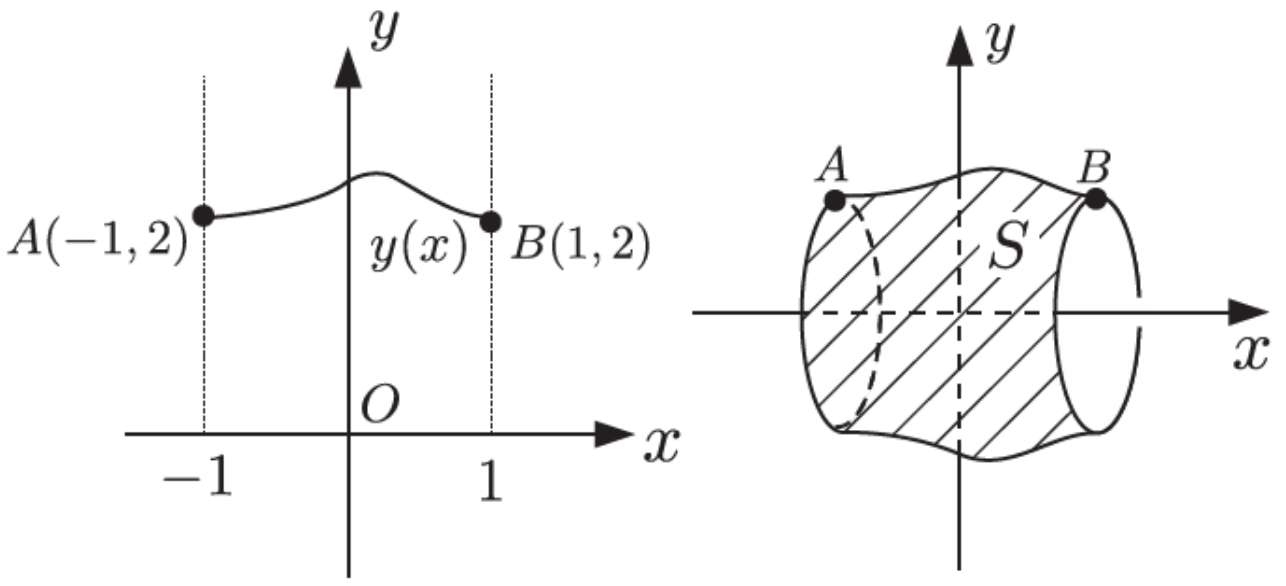
\includegraphics[width=11cm]{figure_2016_01.png}
\end{screen}

\begin{screen}
 (1) 表面積$S$が以下の式で表されることを示せ.
 \begin{align*}
  S &= 2 \pi \int_{-1}^1 F(y,y') \mathrm{d}x,\tag{2.1} \\
  F(y,y') &=y \sqrt{ 1 + \left(y'\right)^2}. \tag{2.2}
 \end{align*}
 ただし$\ds y' = \diff{}{y}{x}$である.
\end{screen}

\begin{screen}
 (2) 曲線$y(x)$は任意の$x$に対して以下のオイラー・ラグランジュ方程式を満たすとする.
 \begin{align*}
  \pdiff{}{F}{y} - \diff{}{}{x}\pdiff{}{F}{y'} = 0. \tag{2.3}
 \end{align*}
 $\ds \diff{}{F}{x}$と式(2.3)を考えることで,以下の関係式が成り立つことを示せ.
 \begin{align*}
  F - y'\pdiff{}{F}{y'} = c. \tag{2.4}
 \end{align*}
 ただし$c$はある定数である.
\end{screen}

\begin{screen}
 (3) 曲線 $y(x)$ が満たすべき微分方程式を$y,y',c$を用いて表わせ.
\end{screen}


\begin{screen}
 (4) 曲線 $y(x)$ を $x$ と $c$ を用いて表わせ.また,定数 $c$ が満たすべき方程式を求めよ.
\end{screen}

\section{}



\end{document}
